% !TeX root = ../main.tex
% Add the above to each chapter to make compiling the PDF easier in some editors.

\chapter{Background}\label{chapter:background}
In this chapter, the theoretical background of time-reversal imaging and rays as model for electromagnetic waves according to Maxwell's equations is presented.
These two concepts are essential for understanding the time-reversal imaging process proposed in this thesis and its underlying physical principles. 

\section{Time-Reversal of the Electromagnetic Field}
\subsection{Time-Reversal Invariance of Physical Laws}
The evolution of a physical system in time can be described by a trajectory \(s(t) \in \mathbb{P}\) in a state-space \(\mathbb{P}\).
This state-space is a high-dimensional space, where each dimension represents a physical property (e.g.~mass, velocity, kinetic energy etc.) of each component of the system.
It should not be confused with the physical space.
In general the time-reversal transformation consists of two components~\parencite{roberts_reversing_2022}.
First, the trajectory \(s(t)\) has to be time-reversed by \(s(t) \mapsto s(-t)\).
This means, that the sequence of the states is reversed with respect to time.
This alone is not sufficient as the properties of the states have to be time-reversed as well.
In a second step, a time-reversal operator has to be applied to each individual instantaneous state \(s(t) \mapsto \mathcal{T}s(t)\), e.g.\ a ball with velocity to the right would become a ball with velocity to the left.
The time-reversal operator acts by either reversing (momentum) or preserving (kinetic energy) the properties.
In summary, time reversing the curve \(s(t)\) results in the curve \(r(t)=\mathcal{T}s(-t)\). 
As \(s(t)\) is an observable trajectory in the physical world, it is a solution to the equations given by the laws that describe the system. 
A law being time-reversal invariant, therefore implies that the time-reversed curve \(r(t)\) is also a solution to this law~\parencite{roberts_time_2021}.

For a more hands-on example, imagine filming a ball that is influenced by gravity while flying through a vacuum.
Newtons second law \({F}=m \cdot {a}\) is time-reversal invariant. 
This means the film can be played backwards and the trajectory of the ball will still follow Newtons second law.
An example for a non time-reversal invariant law is the second law of thermodynamics, which states that the entropy of an isolated system never decreases.
This means, that a film of a gas spreading out in a room played backwards would not comply to this law, as the entropy of the system in the backwards film actually decreases by time.

\begin{figure}[ht]
    \begin{minipage}[b]{0.45\textwidth}
        \centering
        \begin{subfigure}[b]{\textwidth}
            \centering
            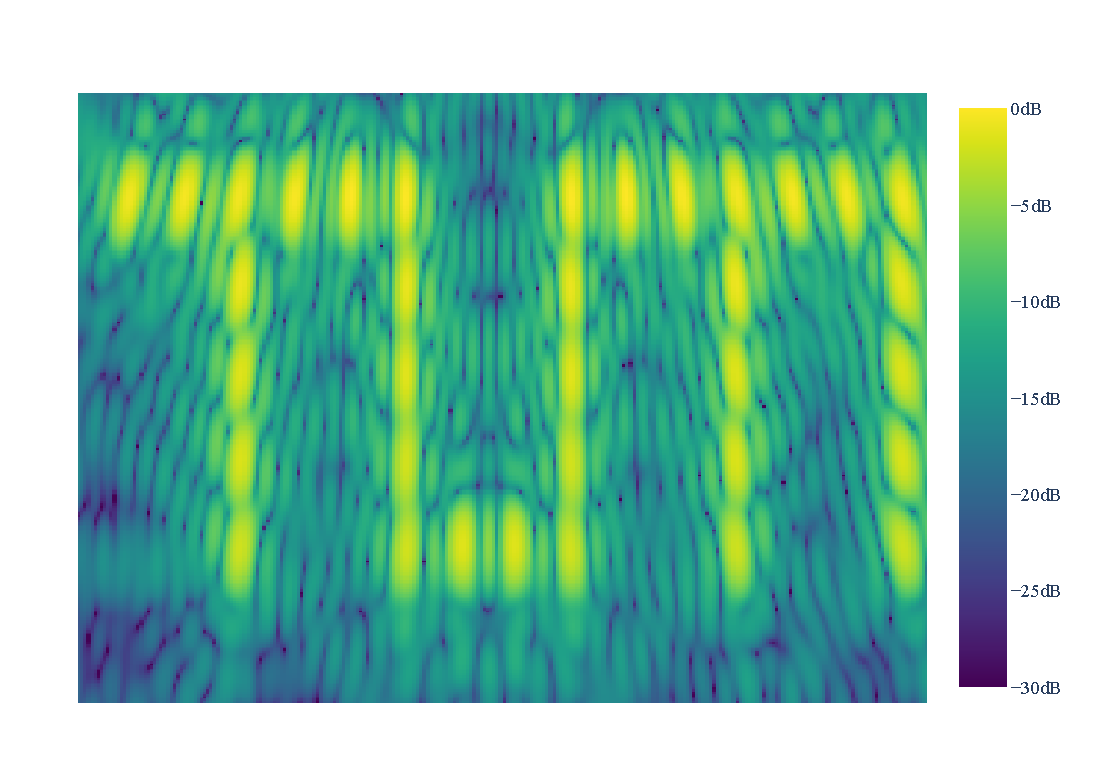
\includegraphics[page=1, width=\textwidth]{figures/pure_los.pdf}
        \end{subfigure}
        
        \begin{subfigure}[b]{\textwidth}
            \centering
            \includegraphics[page=2, width=\textwidth]{figures/pure_los.pdf}
        \end{subfigure}
        \caption{First figure}\label{fig:figure1}
    \end{minipage}
    \hfill
    \begin{minipage}[b]{0.45\textwidth}
        \centering
        \begin{subfigure}[b]{\textwidth}
            \centering
            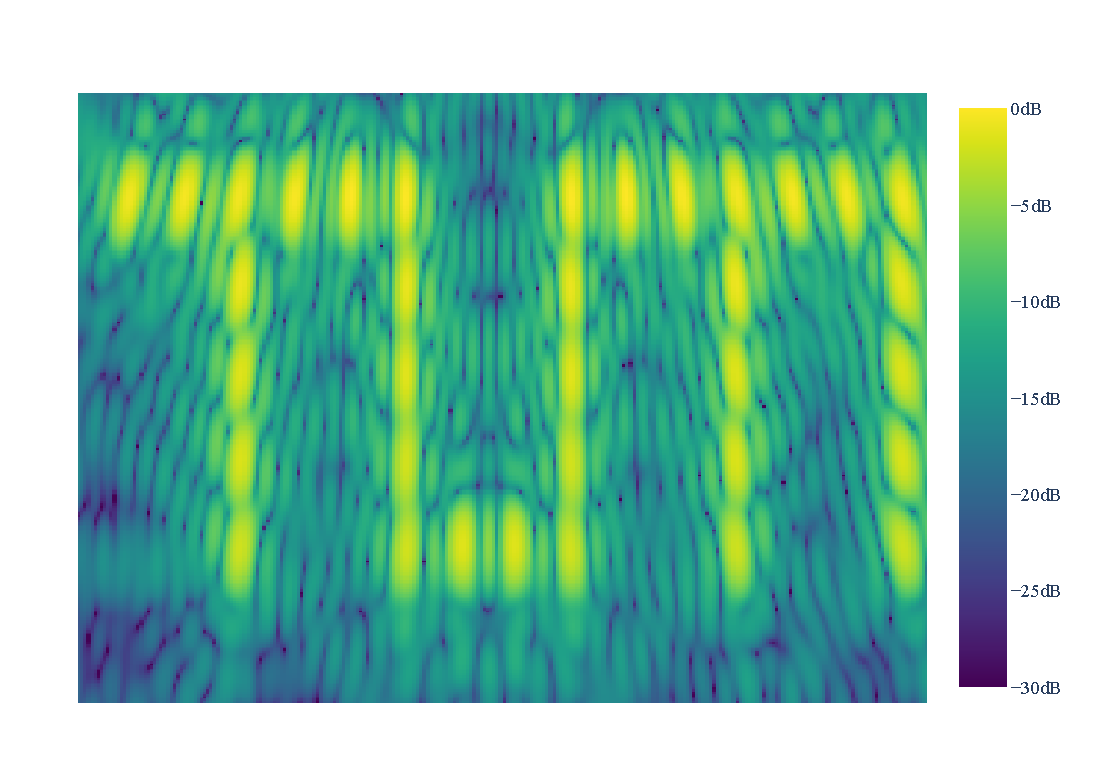
\includegraphics[page=1, width=\textwidth]{figures/pure_los.pdf}
        \end{subfigure}
        
        \begin{subfigure}[b]{\textwidth}
            \centering
            \includegraphics[page=2, width=\textwidth]{figures/pure_los.pdf}
        \end{subfigure}
        \caption{Second figure}\label{fig:figure2}
    \end{minipage}
\end{figure}

\subsection{Time-Reversal Invariance of Maxwell's Equations}
Maxwell's equations formulate the foundations of classical electromagnetism.
They relate the electric field \(\bm{E}\), the electric displacement field \(\bm{D}\), the magnetic field \(\bm{H}\) and the magnetic flux density \(\bm{B}\)  by the following equations, where \(\rho \) and \({\bm{J}}\) denote the electric charge and current densities:
\begin{align}
    \begin{split}
        \nabla \cdot \bm{D} &= \rho \\
        \nabla \times \bm{E} &= -\frac{\partial \bm{B}}{\partial t}
    \end{split}
    &
    \begin{split}
        \nabla \cdot \bm{B} &= 0 \\
        \nabla \times \bm{H} &= \bm{J} + \frac{\partial \bm{D}}{\partial t}
    \end{split}
\end{align}
Generally \(\bm{E}\) and \(\bm{D}\) are related by the electric permittivity \(\varepsilon \), while \(\bm{H}\) and \(\bm{B}\) are related by the magnetic permeability \(\mu \).
In this paper only time-invariant, reciprocal and anisotropic media are considered, which means that the permittivity \(\varepsilon \) and the permeability \(\mu \) are hermitian tensors~\parencite{krowne_electromagnetic_1984}.
This leads to a reduced form of Maxwell's equations, where the electric field \(\bm{E}\) and the magnetic field \(\bm{H}\) are related by
\begin{align}
    \begin{split}
        \nabla \cdot (\varepsilon \bm{E}) &= \rho \\
        \nabla \times \bm{E} &= -\mu \frac{\partial \bm{H}}{\partial t}
    \end{split}
    &
    \begin{split}
        \nabla \cdot (\mu \bm{H}) &= 0 \\
        \nabla \times \bm{H} &= \bm{J} + \varepsilon \frac{\partial \bm{E}}{\partial t}
    \end{split}
\end{align}

For the time-reversal of these equations, one first has to understand, how the time-reversal operator \(\mathcal{T}\) acts on the fields \(\bm{E}\) and \(\bm{H}\).
Taking into account, that the Poynting vector \(\bm{S} = \bm{E} \times \bm{H}\) is a measure for the energy flow of the electromagnetic field, the time-reversal of these fields has to be chosen in a way that the Poynting vector is reversed as well.
This means, that either \(\bm{E}\) or \(\bm{H}\), but not both, have to be reversed so the Poynting vector changes sign. 
The Maxwell equations remain invariant if the fields and densities are transformed as follows~\parencite{sigwarth_time_2022}:
\begin{align}
    \begin{split}
        \mathcal{T}\bm{E} &= \bm{E} \\
        \mathcal{T}\rho &= \rho \\
    \end{split}
    &
    \begin{split}
        \mathcal{T}\bm{H} &= -\bm{H} \\
        \mathcal{T}{\bm{J}} &= -{\bm{J}}
    \end{split}
\end{align}

An intuitive but not rigorous explanation for this transformation is given by the fact, that the electric field is a measure for the force acting on a charge, while the magnetic field is a measure for the force acting on a moving charge. 
Accordingly if time is reversed, the direction of the charges will revert and hence the magnetic field should revert. 
In contrast there is no reason for a positive charge to become a negative charge and vice versa, so the electric field stays the same.


With the time-reversal operator defined for all components of Maxwell's equations the time-reversal of the electric and magnetic field in the time domain can now be written as
\begin{equation}
    \bm{E}_{\text{TR}}(t) = \bm{E}(-t) \quad \bm{H}_{\text{TR}}(t) = -\bm{H}(-t)
\end{equation}
The fourier transformation of these equations with \(\mathcal{F}\{X(t)\} = \hat{X}(\omega) = \int X(t) \cdot \mathrm{e}^{\mathrm{i}\omega t} \, dt\) leads to
\begin{equation}
    \hat{\bm{E}}_{\text{TR}}(\omega) = \hat{\bm{E}}{(\omega)}^* \quad \hat{\bm{H}}_{\text{TR}}(\omega) = -\hat{\bm{H}}{(\omega)}^*
\end{equation}
where \(^*\) denotes the complex conjugate. 

As only fields in the frequency domain will be considered in the following, the hat is dropped.



\section{Reciprocity and Time-Reversal}\label{sec:math_foundations_em_tr}
In \parencite{de_rosny_theory_2010} the mathematical groundwork for the time-reversal of electromagnetic waves has been laid out.
This section won't cover the derivation of their results, but review them as they represent the starting point of mathematical justification for the time-reversal of electromagnetic waves.

\subsection{The Six-Vector Formalism}
The mentioned paper uses two formalisms.
The electric and magnetic field are combined into the  six-vector \(\psi \) which is defined as
\begin{equation}
    \psi(\bm{r}) = \begin{pmatrix}
        \bm{E}(\bm{r}) \\
        \mathrm{i} \bm{H}(\bm{r})
    \end{pmatrix}
\end{equation}
and a source vector \(q\) is defined as
\begin{equation}
    q(\bm{r}) = \begin{pmatrix}
        -\mathrm{i} \bm{J}(\bm{r}) \\
        m(\bm{r})
    \end{pmatrix}
\end{equation}
with \(\bm{J}\) and \(m\) denoting the electric and magnetic current density vectors.

These vector-distributions are linearly related through the Green's function \(G\) of the system
\begin{equation}
    \psi(\bm{r}) = \int G(\bm{r}, \bm{r}^{\prime}) q(\bm{r}^{\prime}) \, d^3 r^{\prime}
\end{equation}
For improved readability the integral is written in the following way
\begin{equation}
    \int G(\bm{r}, \bm{r}^{\prime}) q(\bm{r}^{\prime}) \, d^3 r^{\prime} = [G(\bm{r}) q]
\end{equation}

The above definitions imply that the time-reversal operator \(\mathcal{T}\) acts on the six-vector and the source vector by complex conjugation.
\begin{align}
    \mathcal{T}\psi &= \psi^* \\
    \mathcal{T}q &= q^*
\end{align}

\subsection{The Electromagnetic Time-Reversal Equation}
Under the assumption of a reciprocal environment (\(\varepsilon \) and \(\mu \) are hermitian) the following equation is derived in \parencite{de_rosny_theory_2010}:
\begin{equation}\label{time-reversal-equation}
    \begin{aligned}
    & \underbrace{\oint_{\delta \Gamma} G(\bm{r}^{\prime}, \bm{r})\left(\bm{n}\left(\bm{r}^{\prime}\right) \times\left[G^*\left(\bm{r}^{\prime}\right) q^*\right]\right) d^2 r^{\prime}}_{\psi_S(\bm{r})} \\
    &=\underbrace{[G^*(\bm{r}) q^*] - [G(\bm{r}) q^*]}_{\psi_V(\bm{r})}
    \end{aligned}
\end{equation}
Since \([G^*(\bm{r}) q^*] = \psi^*(\bm{r}) = \mathcal{T}\psi(\bm{r})\), the left-hand side \(\psi_S(\bm{r})\) can be interpreted as a procedure of four steps:
\begin{enumerate}
    \item Measure the electromagnetic field \(\psi \) at the surface \(\delta \Gamma \).\ (\(\oint_{\delta \Gamma} \ldots  (\ldots \times \psi^*(\bm{r}^{\prime})) d^2 r^{\prime}\))
    \item Time-reverse these measurements.\ (\(\psi^*(\bm{r}^{\prime}) = \mathcal{T}\psi(\bm{r}^{\prime})\))
    \item Deduce a source distribution \(q_{\text{TR}}\) from these time-reversed measurements on the surface \(\delta \Gamma \) according to the normal vector of the surface.\ (\(q_{\text{TR}}(\bm{r}^{\prime}) = \bm{n}(\bm{r}^{\prime}) \times \mathcal{T}\psi(\bm{r}^{\prime})\))
    \item Calculate the electromagnetic field \(\psi_S(\bm{r})\) generated by this source distribution.\ (\(\psi_S(\bm{r}) = \oint_{\delta \Gamma} G(\bm{r}^{\prime}, \bm{r}) q_{\text{TR}}(\bm{r}^{\prime})\))
\end{enumerate}
The electromagnetic time-reversal equation~\eqref{time-reversal-equation} then states that this field \(\psi_S(\bm{r})\) is equal to the time-reversed field \(\psi_{\text{TR}}(\bm{r}) = [G^*(\bm{r}) q^*]\) minus a diverging field \(A(\bm{r}) = [G(\bm{r}) q^*]\).
\begin{equation}
    \psi_S(\bm{r}) = \psi_{\text{TR}}(\bm{r}) - A(\bm{r})
\end{equation}
Further investigation of \(A\) shows that it is equal to the field generated by the time-reversed sources.
As the sources are initially turned off, their time-reversed excitation and thus the field \(A\) eventually goes to zero.

In conclusion \parencite{de_rosny_theory_2010} proves that it is possible to compute or recreate the time-reversed version of an electromagnetic field \(\psi_{\text{TR}}\) inside of a medium \(\Gamma \) by measuring the field \(\psi \) at the surface \(\delta \Gamma \), applying the time-reversal operator \(\mathcal{T}\) to these measurements and emitting the resulting sources back into \(\Gamma \).



\section{Time-Reversal Imaging}
This section is dedicated to the explanation of how time-reversal is used for imaging through inverse scattering.
Inverse scattering focuses on identifying the characteristics of an unknown scatterer, including its form, location, and material composition, based on the information obtained from measured scattered fields.
The focus of this thesis is on the localization of passive targets, which are scatterers that do not emit any electromagnetic waves themselves.
This problem is closely related to active-source localization, as the scattered field produced by passive targets can be interpreted as the radiated field from a source at the scatterer location.~\parencite{chen_computational_2018}

\subsection{Active-Source Localization}
Assuming that \(N\) point-sources, denoted as \(q_i(\omega)\), are located at positions \(\bm{r}_i\), the source-distribution \(q(\bm{r}, \omega)\) is obtained, with \(\delta(\bm{r}) \) denoting the dirac delta-function.
\begin{equation}
    q(\bm{r}, \omega) = \sum_{i=1}^{N} \delta(\bm{r} - \bm{r}_i) \cdot q_i(\omega)
\end{equation}
To explain how the described time-reversal process can be used for active-source localization, a signal theory approach is taken.
To do this the medium is modelled as a reciprocal LTI-System.
Now the propagation of an electromagnetic wave-signal \(\psi(\bm{r}, \omega )\) from a source \(q_a(\omega )\) at \(\bm{r}_a\) to a receiver at \(\bm{r}_b\) can be reduced to a simple input-output system with the transfer function \(H_{a\rightarrow b}(\omega) = G(\bm{r}_a, \bm{r}_b, \omega)\).
\begin{equation}
    \psi(\bm{r}_b, \omega) = H_{a\rightarrow b}(\omega) \cdot q_a(\omega)
\end{equation}
This can be applied to the whole source distribution \(q(\bm{r}, \omega)\) to obtain the wave-signal at the receiver \(\bm{j}\).
\begin{equation}
    \psi(\bm{r_j}, \omega) = \sum_{i=1}^{N} H_{i\rightarrow j}(\omega) \cdot q_i(\omega)
\end{equation}
From this wave-signal, an equivalent source \(p_j(\omega)\) can be deduced by applying the measurement operator \(\mathcal{M}\). This is done at all \(M\) receivers at the locations \(\bm{r}_j\).  
\begin{equation}
    p_j(\omega) = \mathcal{M} \psi(\bm{r}_j, \omega)
\end{equation}
Time-reversing (complex-conjugating) the measured sources at all the receivers and remitting them will result in the wave-signal distribution \(\psi_{\text{TR}}(\bm{r}_x, \omega)\) which is again measured with \(\mathcal{M}\)
\begin{equation}\label{signal-time-reversal}
    \mathcal{M} \psi_{\text{TR}}(\bm{r}_x, \omega) = \sum_{j=1}^{M} \mathcal{M} H_{j\rightarrow x}(\omega ) \cdot p_j^*(\omega) = \sum_{j=1}^{M} \sum_{i=1}^{N} \mathcal{M} H_{j\rightarrow x}(\omega) \cdot \mathcal{M}^* \bm{H}^*_{i\rightarrow j}(\omega) \cdot q^*_i(\omega)
\end{equation}
At this point it should be mentioned, that the usage of \(\psi \), \(q\) and the relating measurement operator \(\mathcal{M}\) was chosen for consistency with Section~\ref{sec:math_foundations_em_tr}.
In most papers about electromagnetic time-reversal only the electric field \(\bm{E}\) is considered for simplicity.
Then, by substituting \(\bm{E}\) for \(\psi \) and describing the sources \(q_i\) by the electric field \(\bm{E}_i\) they cause at location \(\bm{r}_i\) (i.e.~\(\mathcal{M}=1\)), equation~\eqref{signal-time-reversal} becomes
\begin{equation}\label{electric-time-reversal}
    \bm{E}_{\text{TR}}(\bm{r}_x, \omega) = \sum_{j=1}^{M} \sum_{i=1}^{N} H_{j\rightarrow x}(\omega )  \bm{H}^*_{i\rightarrow j}(\omega) \cdot \bm{E}^*_i(\omega)
\end{equation}
This approach is valid if the receivers are located in the far-field of the sources.
Here the electric and magnetic fields are orthogonal, so it is sufficient to only keep track of the electric field.
Furthermore the deduction of an equivalent source \(q_{\text{TR}}(\bm{r}) = n(\bm{r}) \times \psi^*(\bm{r})\) can be simplified so the electric and magnetic current densities are proportional to the electric and magnetic field respectively~\parencite{de_rosny_theory_2010}:
\begin{equation}
    q_{T R}(\bm{r})= \begin{pmatrix}
        -\mathrm{i} \bm{J}^*(\bm{r}) \\
        m^*(\bm{r})
    \end{pmatrix} =\left(\begin{array}{c}
        \mathrm{i} \bm{E}^*(\bm{r}) / \eta \\
        \eta \bm{H}^*(\bm{r})
        \end{array}\right)
\end{equation}
At any source location \(\bm{r}_k\) equation~\eqref{electric-time-reversal} becomes
\begin{equation}\label{electric-time-reversal-source}
    \bm{E}_{\text{TR}}(\bm{r_k}, \omega) = \underbrace{\sum_{j=1}^{M} H_{j\rightarrow k}(\omega) \bm{H}^*_{k\rightarrow j}(\omega) \cdot \bm{E}^*_k(\omega)}_{\text{Constructive}} + \underbrace{\sum_{\substack{i=1 \\ i \neq k}}^{M} \sum_{i=1}^{N} H_{j\rightarrow x}(\omega ) \bm{H}^*_{i\rightarrow j}(\omega) \cdot \bm{E}^*_i(\omega)}_{\text{Destructive}}
\end{equation}
As mentioned before, the system is reciprocal so \(H_{j\rightarrow k}(\omega )= H_{k\rightarrow j}(\omega )\). 
Therefore the Constructive part is equal to \(|H_k(\omega)|^2 \cdot \bm{E}^*_k(\omega)\), with
\begin{equation}
    |H_k(\omega)|^2 = \sum_{j=1}^{M} |H_{j\rightarrow k}(\omega)|^2
\end{equation}
This means the constructive part reconstructs the time-reversed signal at the source location \(\bm{r_k}\) without any phase distortion (\(\Im \{{|H_k(\omega)|^2}\} = 0\)) and an attenuation factor of \(|H_k(\omega)|^2\).
Conversely the Destructive part is the sum of all cross-terms of the transfer functions \(H_{j\rightarrow k}(\omega)\) and \(H_{i\rightarrow j}(\omega)\) with \(i \neq k\) that will eventually cancel each other out if the number of receivers goes to infinity.

If~\eqref{electric-time-reversal} is evaluated at any non-source location, no Constructive part will arise, hence the time-reversed signal at this location approaches zero.
With this in mind one can see how equation~\eqref{electric-time-reversal} approximates the time-reversed active-source distribution. 
\begin{equation}
    \bm{E}_{\text{TR}}(\bm{r}, \omega) \approx \bm{E}_{\text{TR-source}}(\bm{r}, \omega) =  \sum_{i=1}^{N} \delta(\bm{r}-\bm{r}_i) \cdot \bm{E}^*_i(\omega)
\end{equation}

\subsection{Monochromatic Signals}
Although there are quite promising attempts of improving the imaging from the reconstructed time-reversed field by using time-domain techniques, like a correlation-based criteria~\parencite{li_correlation-based_2021}, the focus of this thesis will remain on the frequency-domain using monochromatic signals.
These are defined by their amplitude \(|\bm{E}|\) and phase \(\phi \) at a single frequency \(\omega \) and are usually described by a complex phasor \(\underline{\bm{E}}(\bm{r})\).
\begin{equation}
    \underline{\bm{E}}(\bm{r}) = |\bm{E}(\bm{r})| \cdot \mathrm{e}^{\mathrm{i} \phi(\bm{r})} = |\bm{E}(\bm{r})| \cdot (\cos(\phi(\bm{r})) + \mathrm{i} \sin(\phi(\bm{r})))
\end{equation}
The time-domain representation of the signal at location \(\bm{r}\) is retrieved by taking the real part of the product of the phasor and \(\mathrm{e}^{\mathrm{i} \omega t}\).
\begin{equation}
    \bm{E}(\bm{r}, t) = \Re \{\underline{\bm{E}}(\bm{r}) \cdot \mathrm{e}^{\mathrm{i} \omega t}\} = |\bm{E}(\bm{r})| \cdot \cos(\phi(\bm{r}) + \omega t)
\end{equation}
For the phasor \(\underline{\bm{E}}(\bm{r})\) the time-reversal operator \(\mathcal{T}\) is simply a reflection along the real axis or (in mathematical terms) a negation of the phase.

The propagation of a monochromatic wave-signal along a straight line through a system can be modelled by the phasor rotating counter-clockwise in the complex plane.
How far the phasor is rotated is given by the phase of the system's transfer function \(\bm{H}(\bm{r}_{source}, \bm{r})\).
Reflecting the phasor along the real axis will result in the same phasor as if the initial phasor was rotated clockwise while propagating through the system.
This means the time-reversal procedure for monochromatic-signals consists simply of rotating the phasor back along the path it took.
This way all the measured phasors at the receivers rotated back will align in the source-location and hence interfere constructively, resulting in a maximum of amplitude at this point.  

\vspace{1cm}
In conclusion, measuring the far field with multiple sensors and subsequently calculating the field that would be created by antennas emitting the time-reversed signal from the measured locations will result in an amplitude distribution that is maximal at the source locations.
This will then enable the localization of the sources. 
The corresponding imaging formula for \(N\) measurements \(E_i\) of monochromatic waves of frequency \(\omega \) at the locations \(\bm{r}_i\) is~\parencite{peng_zhang_comparison_2013}
\begin{equation}
    I^{\mathrm{\text{TR}}}\left(\bm{r}_p\right)=|\sum_{i=1}^N E_{i}^* \cdot G\left(\bm{r}_i, \bm{r}_p, \omega\right)|
\end{equation}
In this formula \(G(\bm{r}_i, \bm{r}_p, \omega) = H_{i\rightarrow p}(\omega)\) represents the propagation of the wave from the source \(i\) to the imaging-point \(p\).



\section{The Ray Concept of Electromagnetic Waves}\label{sec:ray-concept}
To calculate the imaging formula one needs to know the transfer-function \(H_{i\rightarrow p}(\omega)\) between every receiver and every imaging-point in the target-domain.
This could be done by full-wave simulations of delta-impulses at the measurement locations.
These simulations are extremely computationally expensive.
For this reason a geometric ray-tracing approach is taken to calculate these channel characteristics.
The following section will discuss the connection between Maxwell's equations and geometrical optics, to justify the use of rays for the calculation of the transfer-function, if the wavelength \(\lambda \sim \omega^{-1} \) is small enough.

\subsection{Deriving the Eikonal Equation from Maxwell's Equations}
The following argumentation is based on~\parencite{born_geometrische_1933} and~\parencite{sommerfeld_anwendung_1911}.
Consider a source-free (\(q(\bm{r}) = \bm{J}(\bm{r}) = 0\)) and isotropic (\(\varepsilon(\bm{r}) = \varepsilon_0 \cdot \varepsilon_r(\bm{r})\) and \(\mu(\bm{r}) = \mu_0 \cdot \mu_r(\bm{r}) \)) medium with no free charges (\(\nabla \cdot \bm{E} = 0\)).
Maxwell's equations can then be further simplified to
\makeatletter
\newcommand\Label[1]{&\refstepcounter{equation} (\theequation)\ltx@label{#1}&}
\makeatother
\begin{align*}
    \nabla \cdot \bm{E} &= 0 \Label{eq:electricdivergence} & \nabla \cdot \bm{H} &= 0 \Label{eq:magenticdivergence}\\
    \nabla \times \bm{E} &= -\mu \frac{\partial \bm{H}}{\partial t} \Label{eq:electriccurl} & \nabla \times \bm{H} &= \varepsilon \frac{\partial \bm{E}}{\partial t}\Label{eq:magneticcurl}
\end{align*}
Taking the curl of equation~\eqref{eq:electriccurl} and differentiating~\eqref{eq:magneticcurl} with respect to time yields
\begin{align}
    \nabla \times (\nabla \times \bm{E}) &= -\mu (\frac{\partial}{\partial t} \nabla \times \bm{H}) \\
    \frac{\partial}{\partial t} \nabla \times \bm{H} &= \varepsilon \frac{\partial}{\partial t^2} \bm{E}
\end{align}
Substituting the second equation into the first one results in
\begin{equation}
    \nabla \times (\nabla \times \bm{E}) = -\mu \varepsilon \frac{\partial^2}{\partial t^2} \bm{E}
\end{equation}
Finally, using Green's vector identity (\(\nabla \times (\nabla \times A) = \nabla(\nabla \cdot A) - \nabla^2 A\)) the wave equation for the electric field is obtained, where \(\nabla^2\) denotes the componential Laplacian operator.
\begin{equation}
    \nabla^2 \bm{E} - \mu \varepsilon \frac{\partial^2}{\partial t^2} \bm{E} = 0
\end{equation}
The same equation can be derived for the magnetic field and holds for each single component \(\phi \) of both fields.
For monochromatic waves of frequency \(\omega \) it can be written in the frequency domain as
\begin{equation}\label{electromagnetic_wave_equation}
    \nabla^2 \phi(\bm{r}) + k_0^2\ n{(\bm{r})}^2 \cdot \phi(\bm{r}) = 0
\end{equation}
with \(k_0 = \omega \sqrt{\mu_0 \varepsilon_0} \) denoting the vacuum wave-number and \(n(\bm{r}) = \sqrt{\varepsilon_r(\bm{r}) \mu_r(\bm{r})}\) denoting the refractive index of the medium.

For a monochromatic wave of frequency \(\omega \) the components \(\phi(\bm{r})\) can be described by the complex phasor \(\underline{\phi}(\bm{r}) = A(\bm{r}) \cdot \mathrm{e}^{\mathrm{i} k_0 \cdot \psi(\bm{r})}\) with amplitude \(A(\bm{r})\) and phase \(k_0 \cdot \psi(\bm{r})\).
Equation~\eqref{electromagnetic_wave_equation} then converts to 
\begin{equation}\label{electromagnetic_wave_equation_complex}
    \nabla^2 A(\bm{r}) + 2\mathrm{i}k_0 \cdot \nabla A(\bm{r}) \nabla \psi(\bm{r}) + k_0^2 A(\bm{r}) \cdot ({n(\bm{r})}^2 - {(\nabla \psi(\bm{r}))}^2) = 0
\end{equation}
with a more detailed derivation in~\ref{derivation}

The transition from physical waves to geometrical optics is marked by the limit of \(k_0 \sim  \lambda^{-1} \rightarrow \infty \).
Dividing~\eqref{electromagnetic_wave_equation_complex} by \(k_0^2 A(\bm{r})\) and assuming that the amplitude is slowly varying, the limit \(k_0 \rightarrow \infty \) yields the Eikonal equation.
\begin{equation}
    {n(\bm{r})}^2 - {(\nabla \psi(\bm{r}))}^2 = 0 \quad \Leftrightarrow \quad n(\bm{r}) = |\nabla \psi(\bm{r})|
\end{equation}


\subsection{The Differential Equation of Rays}
Wavefronts are surfaces of constant phase \(\psi(\bm{r})\).
Rays are defined as the orthogonal trajectories of the wavefronts and can be written as curves
\begin{equation}
    \bm{r}(l) = \bm{r}_0 + \int_{0}^{l} \bm{v}(\bm{r}(l^{\prime})) \, dl^{\prime}
\end{equation}
with the unit-ray-vector \(\bm{v}(\bm{r}) = \frac{\nabla \psi(\bm{r})}{|\nabla \psi(\bm{r})|}\).
Combining the Eikonal equation with the definition of the unit-ray-vector yields
\begin{equation}\label{ray-differential-equation}
    n(\bm{r}) \cdot \bm{v}(\bm{r}) = \nabla \psi(\bm{r})
\end{equation}
Considering the identities \(\nabla(A^2)= 2 \cdot A \cdot \nabla A\) and \(\nabla[{(\nabla A)}^2] = 2 \cdot \nabla A \cdot \nabla^2 A\) and deriving equation~\eqref{ray-differential-equation} with respect to \(l\) results in the differential equation of rays~\parencite{born_foundations_1999}
\begin{align}
    \frac{d}{dl}(n(\bm{r}) \cdot \bm{v}(\bm{r})) &= \frac{d}{dl}(\nabla \psi(\bm{r})) = \nabla^2 \psi(\bm{r}) \cdot \frac{d\bm{r}}{dl} \nonumber \\
    &= \nabla^2 \psi(\bm{r}) \cdot \bm{v}(\bm{r}) = \nabla^2 \psi(\bm{r}) \cdot \nabla \psi(\bm{r}) \cdot \frac{1}{n(\bm{r})} \nonumber \\
    &= \frac{1}{2n(\bm{r})} \cdot \nabla[{(\nabla \psi)}^2] = \frac{1}{2n(\bm{r})} \cdot \nabla({n(\bm{r})}^2) \nonumber \\
    &= \nabla n(\bm{r})
\end{align}
For a ray in a homogenous medium, i.e.~\(n(\bm{r}) = n_0\), this equation becomes
\begin{equation}
    n_0 \cdot \frac{d}{dl}\bm{v}(\bm{r}) = 0
\end{equation}
so the unit-ray-vector is a constant and hence the ray is a straight line.
\begin{equation}
    \bm{r}(l) = \bm{r}_0 + l \cdot \bm{v}_0
\end{equation}


\subsection{Refraction and Reflection at Plane Interfaces}
At a plane interface \(\Gamma \) of two homogenous media (\(\Lambda_1\) and \(\Lambda_2\)) with different refractive indices \(n_1\) and \(n_2\), the differential equation of rays must be fulfilled.
An incident ray with unit-vector \(\bm{v}_1\) and the transmitted ray with unit-vector \(\bm{v}_2\) therefore satisfy the following conditions at any point on the interface.
\begin{equation}
    n_1 \cdot \bm{v}_1 = \nabla \psi|_{r \in \Lambda_1 } \quad n_2 \cdot \bm{v}_2 = \nabla \psi|_{r \in \Lambda_2 } 
\end{equation}
The closed integral over a gradient field is always zero.
For any rectangular curve \(C\) (width \(w\) and height \(h\)) where the edges of length \(w\) are tangential to \(\Gamma \) the integral of the gradient field must still be zero.
The tangential parts of the curve are either in \(\Lambda_1\) or \(\Lambda_2\).
Taking the limit of \(h \to 0\) then results in~\parencite{born_foundations_1999}
\begin{equation}
    \lim_{h \to 0} \oint_C \nabla \psi \cdot d\bm{r} = \int_{0}^{w} \nabla \psi|_{r \in \Lambda_1 } \cdot \bm{t} \, dw' + \int_{0}^{w} \nabla \psi|_{r \in \Lambda_2 } \cdot (-\bm{t}) \, dw' = 0
\end{equation}
This means that the tangential components of the ray-vectors \(n \cdot \bm{v}\) are continuous across the interface.
\begin{equation}
    (n_2 \bm{v}_2 - n_1 \bm{v}_1) \cdot \bm{t} = 0
\end{equation}
With \(\bm{t} = \bm{b} \times \bm{n}\) where \(\bm{n}\) is the normal vector of \(\Gamma \) and \(\bm{b}\) is the normal vector of the plane where \(C\) lies this becomes
\begin{equation}
    \bm{b} \cdot [\bm{n} \times (n_2 \bm{v}_2 - n_1 \bm{v}_1)] = 0
\end{equation}
This equation holds for an arbitrary orientation of the curve \(C\) as long as the edges of length \(w\) are completely in either \(\Lambda_1\) or \(\Lambda_2\).
This implies that \(\bm{b}\) can be chosen arbitrarily as long as \(\bm{t} = \bm{b} \times \bm{n}\) still holds.
With this in mind and \(\theta_1\),\(\theta_2\) denoting the angles of \(\bm{v}_1\),\(\bm{v}_2\) with the surface normal \(\bm{n}\), Snell's law is retrieved
\begin{equation}
    \bm{n} \times (n_2\bm{v}_2) - \bm{n} \times (n_1\bm{v}_1) = 0 \quad \Rightarrow \quad n_1 \sin(\theta_1) = n_2 \sin(\theta_2)
\end{equation}

It is known, that at the transition between two media with different refractive indices there is always a refracted as well as a reflected wave.
The reflected wave is in the same medium as the incident wave, which leads to the law of specular reflection.
\begin{equation}
    \sin(\theta_{inc}) = \sin(\theta_{ref})
\end{equation}


\subsection{Phase and Amplitude Propagation along Ray-Paths}
According to the definition of the ray-path \(\bm{r}(l)\) and the Eikonal equation, the derivation of the phase \(k_0 \cdot \psi(\bm{r})\) of a wave along this path is always equal to \(k_0\) times the refractive index \(n(\bm{r})\) so the phase propagation can be written as
\begin{equation}
    k_0 \cdot \psi(\bm{r}(l)) = k_0 \cdot \int_{0}^{l} n(\bm{r}(l^{\prime})) \, dl^{\prime}
\end{equation}
In a homogenous medium this simplifies to
\begin{equation}
    k_0 \cdot \psi(\bm{r}(l)) = k_0 \cdot n \cdot l
\end{equation}

The Amplitude on the other hand has a much more complex behavior even along ray-paths.
For a single point-source in a lossless medium the radiated energy is conserved so the integral over the Poynting-Vector \(S\) over a sphere \(\mathcal{S} \) of radius \(r\) must be independent of \(r\).
\begin{equation}
    \int_\mathcal{S}  S \cdot \bm{n} \, d\Omega = |S| \cdot 4\pi r^2 = \text{const}
\end{equation}
This means, the amplitude of \(S\) is inversely proportional to the square of the distance from the source.
The amplitude of the Poynting-Vector is furthermore proportional to the amplitude of the electric field squared, which concludes that the amplitude of the electric field is inversely proportional to the distance from the source.
\begin{equation}
    |\bm{E}| \propto \frac{1}{r}
\end{equation}
In scenarios like the reflection at interfaces, the amplitude and direction of the electric field vector can be calculated by the Fresnel equations, where the polarization of the field is considered as well.
For our case it is sufficient to model a reflective surface with a virtual source that is placed in the mirrored position of the original source with respect to the surface, so the reflected ray's amplitude keeps decreasing with \(\frac{1}{l}\), where \(l\) is the distance from the virtual source.
If the scenario is even more complex, for example curved reflective surfaces, or sharp edges, a more sophisticated model would be needed.

With these limitations in mind, the propagation of the electric field along a straight ray-path \(\bm{r}(l)\) from a source \(\underline{\bm{E}}_0\) through a homogenous medium (refractive index \(n\)), with \(l\) denoting the distance from the source, can be described as
\begin{equation} \label{eq:field-along-ray-path}
    \underline{\bm{E}}(l) = \frac{1}{1 + l} \cdot \underline{\bm{E}}_0 \cdot \mathrm{e}^{\mathrm{i} k_0 \cdot n \cdot l}
\end{equation}
The factor \(\frac{1}{1 + l}\) is chosen so the decay of the amplitude is inversely proportional to \(l\) and  \(\underline{\bm{E}}(0) = \underline{\bm{E}}_0 \)




\subsubsection{Derivation}\label{derivation}
Consider these identities
\begin{align}
    \nabla^2 (a \cdot b) &= \nabla^2 a \cdot b + 2 (\nabla a \nabla b) + a \nabla^2 b, \\
    \nabla \mathrm{e}^{\mathrm{i} k_0 \cdot \psi(\bm{r})} &= i k_0 \cdot \nabla \psi(\bm{r}) \cdot \mathrm{e}^{\mathrm{i} k_0 \cdot \psi(\bm{r})}, \\
    \nabla^2 \mathrm{e}^{\mathrm{i} k_0 \cdot \psi(\bm{r})} &= - k_0^2 \cdot {(\nabla \psi(\bm{r}))}^2 \cdot \mathrm{e}^{\mathrm{i} k_0 \cdot \psi(\bm{r})}.
\end{align}
which lead to
\begin{gather}
    \nabla^2 (A(\bm{r}) \cdot \mathrm{e}^{\mathrm{i}k_0 \cdot \psi(\bm{r})}) \nonumber \\
    = (\nabla^2 A(\bm{r}) + 2\mathrm{i}k_0 \cdot \nabla A(\bm{r}) \nabla \psi(\bm{r}) - k_0^2 \cdot (\nabla \psi(\bm{r}))) \cdot \mathrm{e}^{\mathrm{i}k_0 \cdot \psi(\bm{r})}
\end{gather}
This results in the following equivalence (\(\underline{\phi}(\bm{r}) = A(\bm{r}) \cdot \mathrm{e}^{\mathrm{i}k_0 \cdot \psi(\bm{r})}\))
\begin{gather}
    \nabla^2 \underline{\phi}(\bm{r}) + k_0^2\ n{(\bm{r})}^2 \cdot \underline{\phi}(\bm{r}) \stackrel{!}{=} 0, \\
    \Leftrightarrow \nabla^2 A(\bm{r}) + 2\mathrm{i}k_0 \cdot \nabla A(\bm{r}) \nabla \psi(\bm{r}) + k_0^2 A(\bm{r}) \cdot ({n(\bm{r})}^2 - {(\nabla \psi(\bm{r}))}^2) \stackrel{!}{=} 0.
\end{gather}